\documentclass[compress]{beamer}
%--------------------------------------------------------------------------
% Common packages
%--------------------------------------------------------------------------
\usepackage[english]{babel}
\usepackage{microtype}

\usepackage{graphicx}
\usepackage{hyperref}
\usepackage{xcolor}

\usepackage{amsmath,amsfonts,amssymb}
\usepackage{amsthm}
\usepackage{dsfont}

\usepackage{pgfplots}

\usepackage{empheq}
\usepackage[ruled,vlined,linesnumbered]{algorithm2e}


\newcommand{\N}{\ensuremath{\mathbb{N}}}
\newcommand{\Z}{\ensuremath{\mathbb{Z}}}
\newcommand{\Q}{\ensuremath{\mathbb{Q}}}
\newcommand{\R}{\ensuremath{\mathbb{R}}}

\newcommand{\PP}{\ensuremath{\mathbb{P}}}
\newcommand{\VV}{\ensuremath{\mathbb{V}}}
\newcommand{\FF}{\ensuremath{\mathbb{F}}}




%--------------------------------------------------------------------------
% Load theme
%--------------------------------------------------------------------------
\usetheme{hsrm}

\usepackage{tikz}
\usetikzlibrary{mindmap,backgrounds}

%--------------------------------------------------------------------------
% General presentation settings
%--------------------------------------------------------------------------
\title{Rays-Crashing}
\subtitle{Project Presentation}
\date{January 09, 2016}
\author{Etienne Moutot}
%\institute{}

%--------------------------------------------------------------------------
% Notes settings
%--------------------------------------------------------------------------
\setbeameroption{show notes}

\begin{document}
%--------------------------------------------------------------------------
% Titlepage
%--------------------------------------------------------------------------

\maketitle

%\begin{frame}[plain]
%	\titlepage
%\end{frame}


%--------------------------------------------------------------------------
% Content
%--------------------------------------------------------------------------

%\section*{Surface Reconstruction}

%\subsection{Surface Reconstruction}
\begin{frame}
	\begin{figure}[htp]
	\centering
	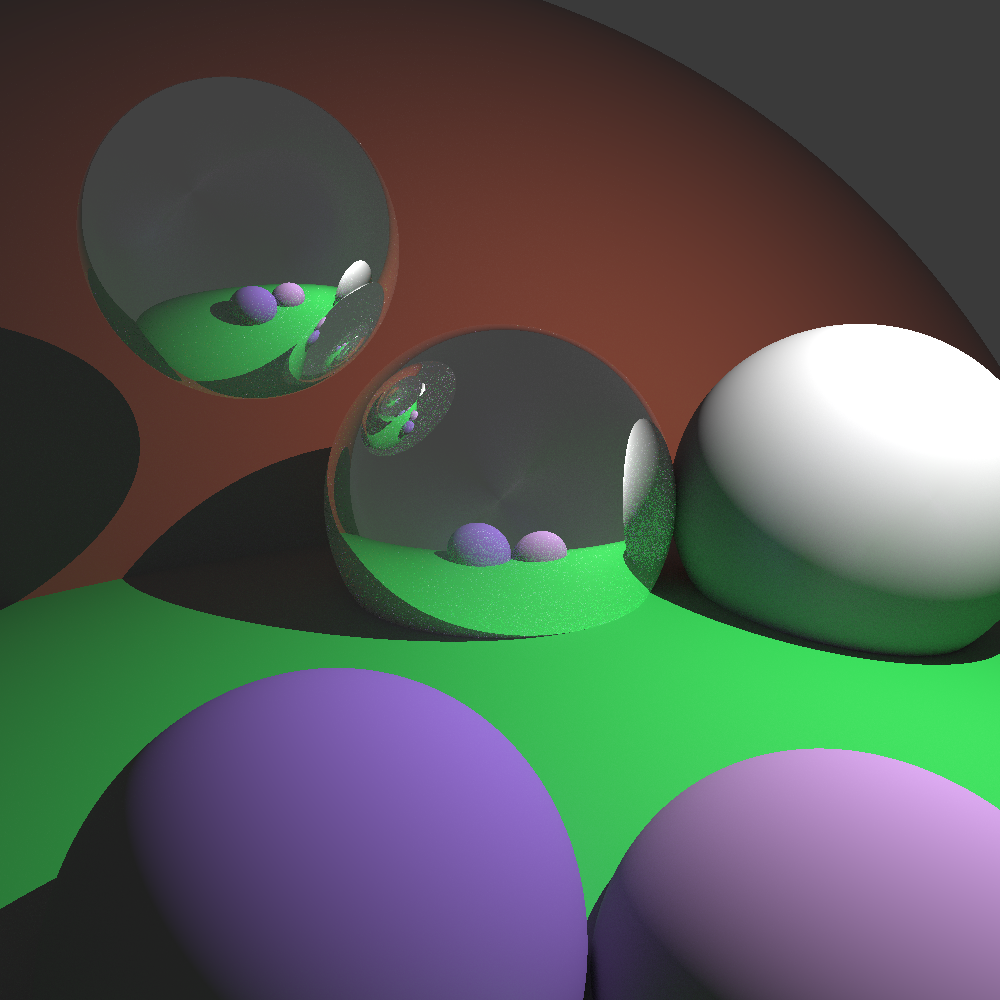
\includegraphics[scale=0.23]{img/ex_1000.png}
	\end{figure}
\end{frame}


% ------------------------------------------------------------
\section{Rays-crashing}

\subsection{rays-crashing}
\begin{frame}{Features}
	\begin{itemize}
  \item Direct lightening
  \item Materials: Diffuse, Specular and Transparent
  \item Indirect lightening using Monte-Carlo method
  \item Parallelization
  \item Gamma correction
\end{itemize}
\end{frame}

\end{document}
